% ==============================================================================
% reports/sections/results/06_03_time_based.tex
% ==============================================================================

\section{Kết quả đánh giá tập kiểm thử theo thời gian}

Sau khi đóng băng cấu hình siêu tham số và lưu vết mã băm trong \texttt{frozen.json}, quy trình thực nghiệm tiến hành mở tập kiểm thử $\Dtest$ đúng một lần duy nhất. Kết quả đánh giá của 3 mô hình trên tập kiểm thử theo thời gian (kịch bản chính theo thời gian có cổng) được thể hiện tại Phần A của Bảng \ref{tab:test_comparison}.

\begin{table}[htbp]
\centering
\caption{Hiệu năng tổng thể trên tập Test đối chuẩn giữa 12 tổ hợp thực nghiệm (Đánh giá sau khi khóa cấu hình).}
\label{tab:test_comparison}
\adjustbox{max width=\textwidth}{%
\begin{tabular}{lllrrrrrrrr}
\toprule
\textbf{Mô hình} & \textbf{Phân tách} & \textbf{Kịch bản} & \textbf{Accuracy} & \textbf{Precision} & \textbf{Recall} & \textbf{F1} & \textbf{AP} & \textbf{ROC-AUC} & \textbf{FTP Rec.} & \textbf{SSH Rec.} \\
\midrule
\multicolumn{11}{l}{\textbf{A. Thực nghiệm Chính: Phân tách theo Thời gian (Time-based Zero-shot)}} \\
Decision Tree & Time & With Port & 0.9740 & 0.0000 & 0.0000 & \textbf{0.0000} & 0.0259 & 0.5000 & \text{N/A} & 0.00\% \\
Random Forest & Time & With Port & 0.9742 & 1.0000 & 0.0019 & \textbf{0.0037} & 0.3591 & 0.7483 & \text{N/A} & 0.19\% \\
XGBoost & Time & With Port & 0.9741 & 0.0000 & 0.0000 & \textbf{0.0000} & 0.0879 & 0.7503 & \text{N/A} & 0.00\% \\
Decision Tree & Time & Without Port & 0.9741 & 0.4375 & 0.0019 & \textbf{0.0037} & 0.0272 & 0.5009 & \text{N/A} & 0.19\% \\
Random Forest & Time & Without Port & 0.9739 & 0.2414 & 0.0038 & \textbf{0.0074} & 0.0268 & 0.4932 & \text{N/A} & 0.38\% \\
XGBoost & Time & Without Port & 0.9740 & 0.2653 & 0.0035 & \textbf{0.0069} & 0.2447 & 0.9304 & \text{N/A} & 0.35\% \\
\midrule
\multicolumn{11}{l}{\textbf{B. Thực nghiệm Đối chứng: Phân tách Ngẫu nhiên (Random Split Control)}} \\
Decision Tree & Random & With Port & 0.9996 & 0.9904 & 0.9980 & \textbf{0.9942} & 0.9963 & 0.9990 & 100.00\% & 99.54\% \\
Random Forest & Random & With Port & 1.0000 & 1.0000 & 0.9993 & \textbf{0.9997} & 1.0000 & 1.0000 & 100.00\% & 99.85\% \\
XGBoost & Random & With Port & 1.0000 & 0.9993 & 1.0000 & \textbf{0.9997} & 1.0000 & 1.0000 & 100.00\% & 100.00\% \\
Decision Tree & Random & Without Port & 0.9989 & 0.9700 & 0.9949 & \textbf{0.9823} & 0.9890 & 0.9974 & 99.69\% & 99.23\% \\
Random Forest & Random & Without Port & 0.9997 & 0.9934 & 0.9954 & \textbf{0.9944} & 0.9994 & 1.0000 & 99.73\% & 99.28\% \\
XGBoost & Random & Without Port & 0.9999 & 0.9980 & 0.9987 & \textbf{0.9984} & 0.9999 & 1.0000 & 99.92\% & 99.79\% \\
\bottomrule
\end{tabular}%
}
\end{table}


Kết quả thực nghiệm ghi nhận sự suy giảm hiệu năng rõ rệt đối với biến thể tấn công mới:
\begin{itemize}
    \item Decision Tree: Đạt $\FOne = \DTTestFOne$, $\Precision = \DTTestPrecision$, $\Recall = \DTTestRecall$, $\AP = \DTTestAP$, $\ROCAUC = \DTTestROCAUC$. Ma trận nhầm lẫn: $TP = \DTTestTP$, $FP = \DTTestFP$, $FN = \DTTestFN$, $TN = \DTTestTN$. Mô hình không nhận diện được mẫu tấn công SSH nào ($\text{SSH Recall} = \DTTestSSHRecall$).
    \item Random Forest: Đạt $\FOne = \RFTestFOne$, $\Precision = \RFTestPrecision$, $\Recall = \RFTestRecall$, $\AP = \RFTestAP$, $\ROCAUC = \RFTestROCAUC$. Ma trận nhầm lẫn: $TP = \RFTestTP$, $FP = \RFTestFP$, $FN = \RFTestFN$, $TN = \RFTestTN$. Mô hình chỉ nhận diện chính xác \RFTestTP\ trên tổng số \DataTestSSH\ flow tấn công SSH, tương ứng với tỷ lệ phát hiện $\text{SSH Recall} = \RFTestSSHRecall$.
    \item XGBoost:
    Đạt $\FOne = \XGBTestFOne$, $\Precision = \XGBTestPrecision$, $\Recall = \XGBTestRecall$, $\AP = \XGBTestAP$, $\ROCAUC = \XGBTestROCAUC$. Ma trận nhầm lẫn gồm $TP = \XGBTestTP$, $FP = \XGBTestFP$, $FN = \XGBTestFN$, $TN = \XGBTestTN$. Tương tự Decision Tree, XGBoost không nhận diện được cuộc tấn công SSH nào ($\text{SSH Recall} = \XGBTestSSHRecall$).
\end{itemize}

Ma trận nhầm lẫn chi tiết của ba mô hình trên tập kiểm thử được trực quan hóa trên Hình \ref{fig:confusion_matrices_detailed}.

\begin{figure}[htbp]
\centering
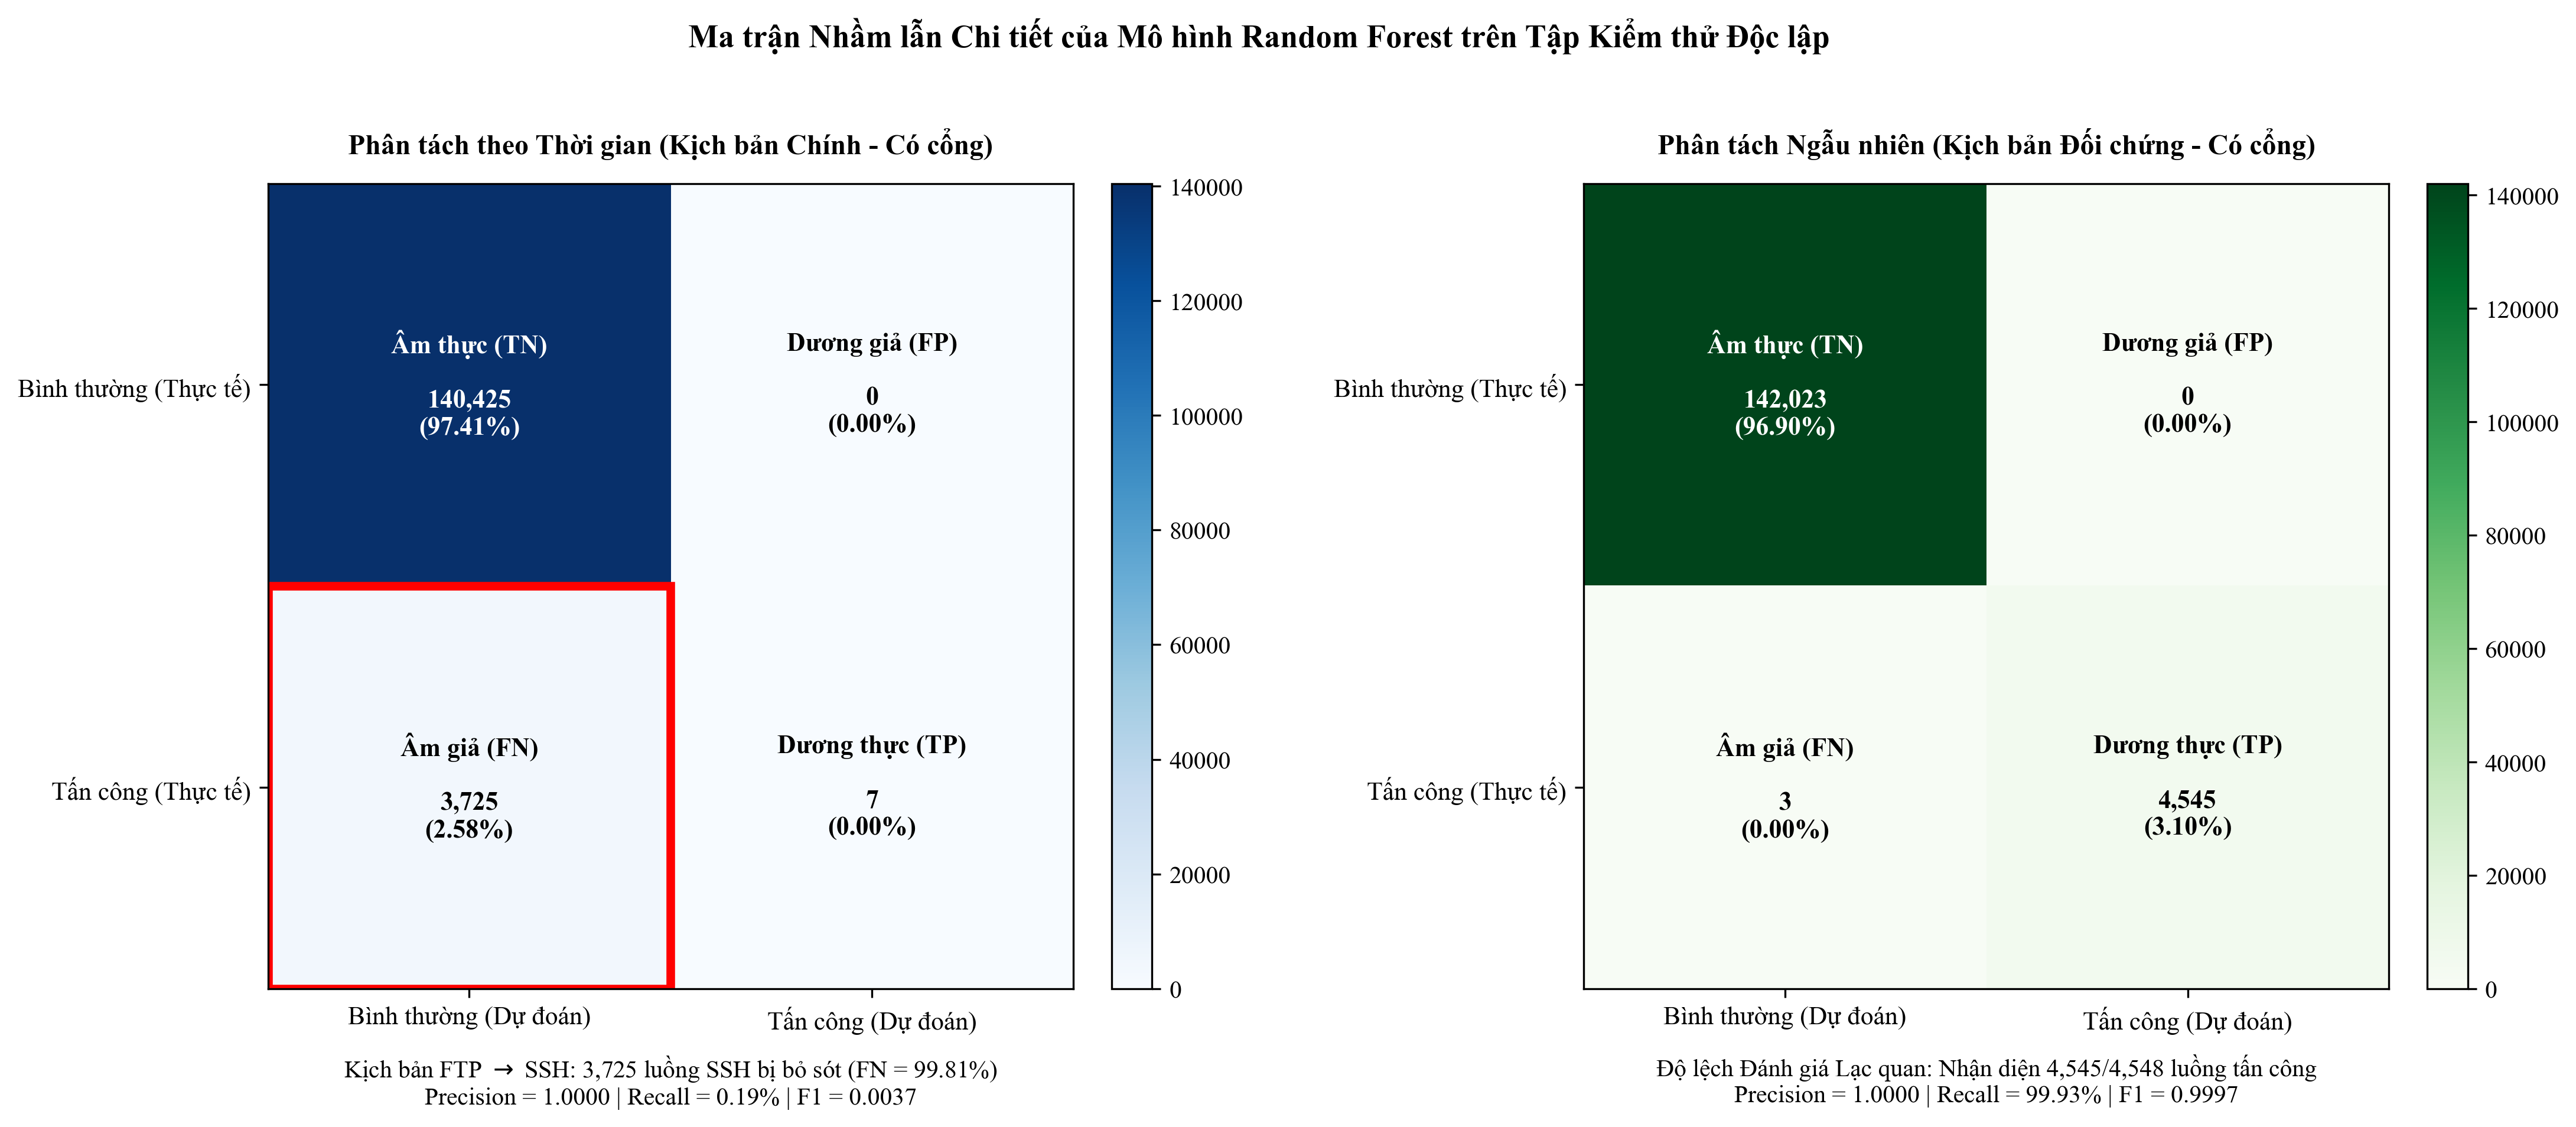
\includegraphics[width=0.92\textwidth]{experiments/figures/03_confusion_matrices_detailed.png}
\caption{Ma trận nhầm lẫn chi tiết của các mô hình trên tập kiểm thử phân tách theo thời gian, thể hiện trực quan tỷ lệ True Positive rất thấp đối với biến thể tấn công SSH.}
\label{fig:confusion_matrices_detailed}
\end{figure}

\noindent\textbf{Ghi nhận về Support và FTP Recall trên tập Test:}
Do tập $\Dtest$ theo thời gian diễn ra từ 14:32 đến 17:00 chiều (chỉ xuất hiện chiến dịch \SSH), số lượng mẫu hỗ trợ của \FTP\ là $0$ ($\text{FTP Support} = 0$). Theo đúng nguyên tắc trung thực học thuật đã đề ra, chỉ số FTP Recall trên tập Test được ghi nhận là N/A (Not Applicable), không gán giá trị 0\% hay 100\%.

\noindent\textbf{Nhận xét kết quả:}
Trong kịch bản đánh giá chính theo thời gian có cổng, Random Forest đạt $\FOne = \RFTestFOne$ với $\text{SSH Recall} = \RFTestSSHRecall$ (\RFTestTP/\DataTestSSH\ flow SSH), trong khi Decision Tree và XGBoost có $\FOne = \DTTestFOne$. Kết quả cho thấy các mô hình học máy dạng cây gặp khó khăn khi áp dụng lên subtype SSH không có trong tập fit của benchmark chuẩn. Tuy nhiên, \DataValidationSSH\ mẫu SSH trong Validation và nhãn của chúng tham gia lựa chọn siêu tham số; vì vậy đây là đánh giá subtype vắng mặt trong tập fit, không phải phép thử zero-shot khép kín từ đầu đến cuối.
